\section{Experiments} \label{sec:experiments}
In this section, we describe our experimental evaluation of four widely used algorithms on real-world datasets and our benchmark. The goal is to assess the quality of the generated $k$-means coresets. On that account, we measure the distortion. In addition, we want to measure how noise reduction affects the coreset quality. For that, we create PCA transformed version for each of the real-world datasets. As the evaluated algorithms are randomized, we repeat each experiment ten times, reporting the mean distortion and variance for different values of $k$.


\subsection{Datasets}
We use three common real-world datasets for evaluating $k$-means coresets 
---
\textit{Census}\footnote{\url{https://archive.ics.uci.edu/ml/datasets/US+Census+Data+(1990)}},
\textit{Covertype}\footnote{https://archive.ics.uci.edu/ml/datasets/covertype}, and 
\textit{Tower}\footnote{\url{http://homepages.uni-paderborn.de/frahling/coremeans.html}}
---
and several instances of the proposed benchmark. 
The \textit{Census} dataset is a small subset of the Public Use Microdata Samples from 1990 US census. It consists of demographic information encoded as 68 categorical attributes of 2,458,285 individuals. \textit{Covertype} is comprised of cartographic descriptions and forest cover type of four wilderness areas in the Roosevelt National Forest of Northern Colorado in the US. It consists of 581,012 records, 54 cartographic variables and one class variable. Although \textit{Covertype} was originally made for classification tasks, it is often used for clustering tasks by removing the class variable~\cite{AckermannMRSLS12}. \textit{Tower} is a 2,560 by 1,920 picture of a tower on a hill where each pixel is represented by a RGB color value. This dataset consists of 4,915,200 rows and 3 columns. To evaluate how denoising effects the quality of the output, we apply SVD on \textit{Census} and \textit{Covertype} using the $k$ largest singular values. Note that we do not reduce the number of dimensions of the original datasets. 


%
\begin{table}
	\begin{center}%\centering
	\caption{The sizes of the real-world datasets used for the experimental evaluation}
	\label{tab:real-world-datasets-overview}
% 	\resizebox{\textwidth}{!}{
	\begin{tabular}{lrr}
		\toprule
        
		    & Data points
		    & Dimensions
            \\
		\midrule
		\textit{Census}
    		& 2,458,285
    		& 68
    		\\
	    \textit{Covertype}
    	    & 581,012
    		& 54
    		\\
        \textit{Tover}
            & 4,915,200
    		& 3
    		\\
		\bottomrule
	\end{tabular}\\
	\end{center}
% 	}
\end{table}

As for the benchmark dataset, instances can be generated via three parameters; the size of clusters $k$, the number of column blocks $\alpha$ and the scaling factor $\beta$. Only parameters $k$ and $\alpha$ determine the size of the dataset. The number of data points in the dataset is given by $n=k^{\alpha}$ and the number of dimensions is $d=\alpha k$. Our aim was to generate instances that roughly match the sizes of the real-world datasets. The chosen parameters values and the corresponding dataset sizes are shown in ~\cref{tab:benchmark-instances-overview}. We generated a set of instances with no scaling i.e., $\beta=1.0$ (referred to as \textit{Benchmark-1.0}) and with maximum scaling; $\beta = 2.0$ (\textit{Benchmark-2.0}).



%
\begin{table}
	\begin{center}%\centering
	\caption{The parameter values and the sizes of the benchmark instances used for the experimental evaluation.}
	\label{tab:benchmark-instances-overview}
% 	\resizebox{\textwidth}{!}{
	\begin{tabular}{rrrr}
		\toprule
        $k$
		    & $\alpha$
		    & Data points
		    & Dimensions
            \\
		\midrule
        10
    		& 6
    		& 1,000,000
    		& 60
    		\\
        20
    		& 5
    		& 3,200,000
    		& 100
    		\\
        30
    		& 4
    		& 810,000
    		& 120
    		\\
        40
    		& 4
    		& 2,560,000
    		& 160
    		\\
        50
    		& 4
    		& 6,250,000
    		& 200
    		\\
		\bottomrule
	\end{tabular}\\
	\end{center}
% 	}
\end{table}

\subsection{Algorithm Parameters}
We followed the same experimental procedure with respect to the choice of parameter values for the algorithms as prior works~\cite{FGSSS13, AckermannMRSLS12}. For the target coreset size, we used $200k$ for all our experiments. On \textit{Census} and \textit{Covertype}, we used $k$ values $\{10, 20, 30, 40, 50\}$, while for \textit{Tower} we used larger cluster sizes $k \in \{20, 40, 60, 80, 100\}$ as in. On the benchmark instances, we settled on $k \in \{10, 20, 30, 40, 50\}$ as a reasonable trade-off between running time and dataset size.



\subsection{Results}

\begin{figure*}
  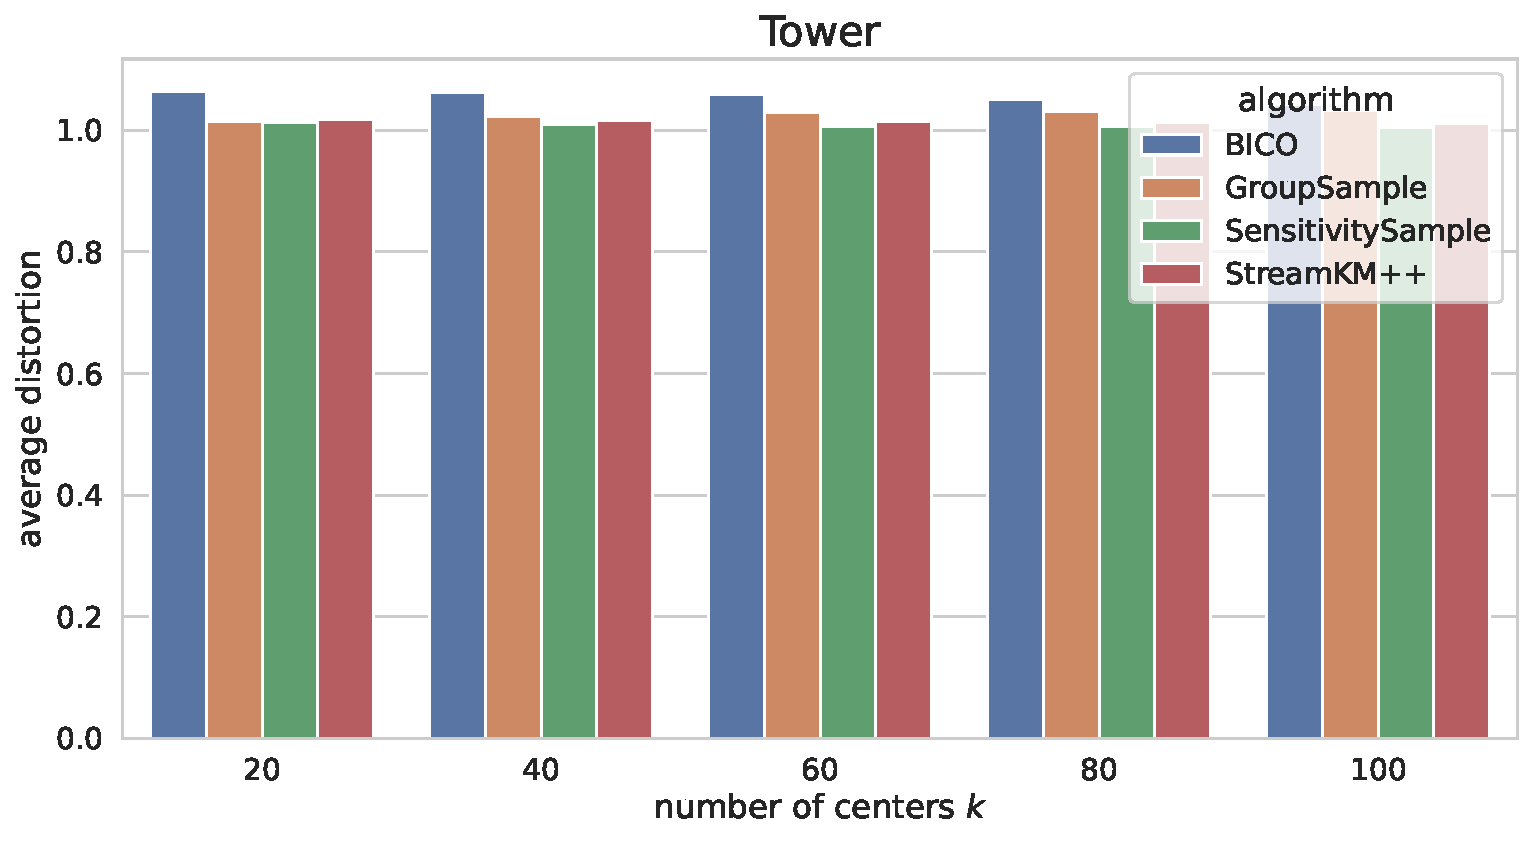
\includegraphics[width=.65\linewidth]{figures/results-Tower.pdf}
  \newline \newline
  \subfloat{
    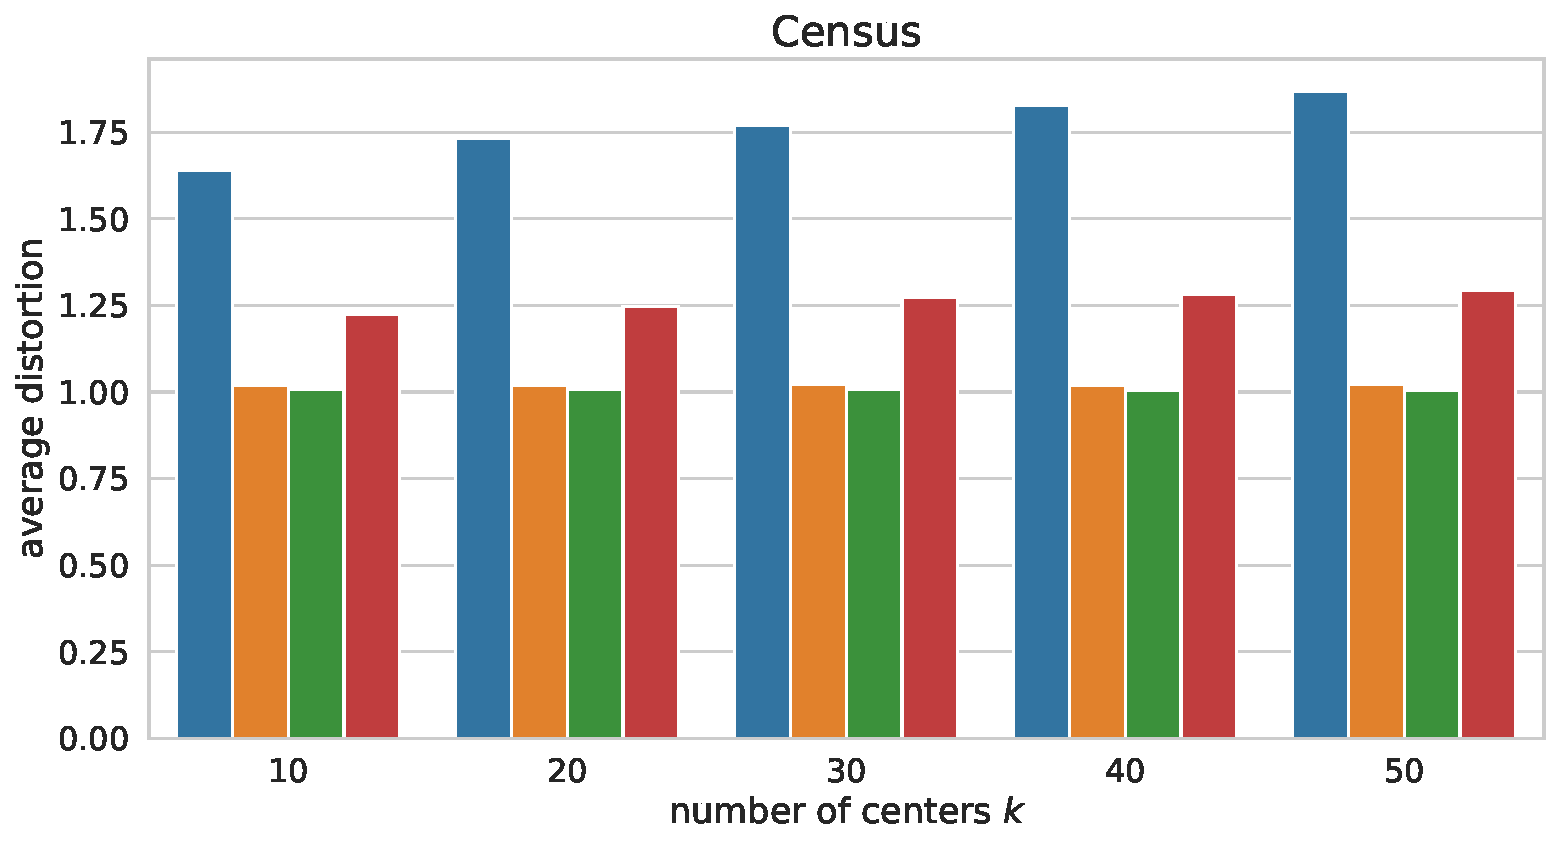
\includegraphics[width=0.5\textwidth]{figures/results-Census.pdf}
  }
  \subfloat{
    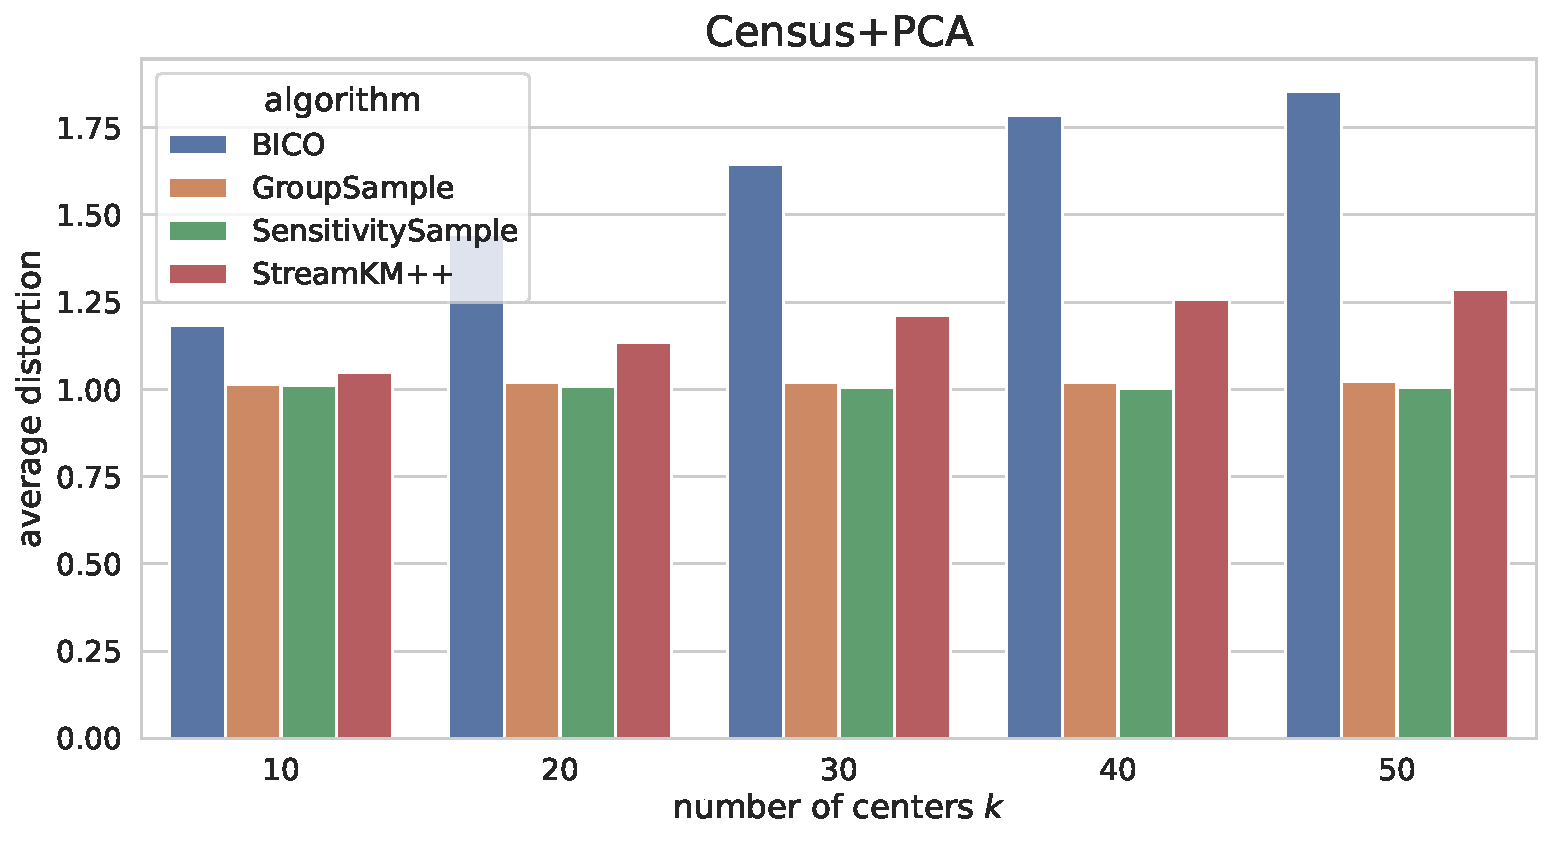
\includegraphics[width=.5\linewidth]{figures/results-Census+PCA.pdf}
  }
  \newline \newline
  \subfloat{
    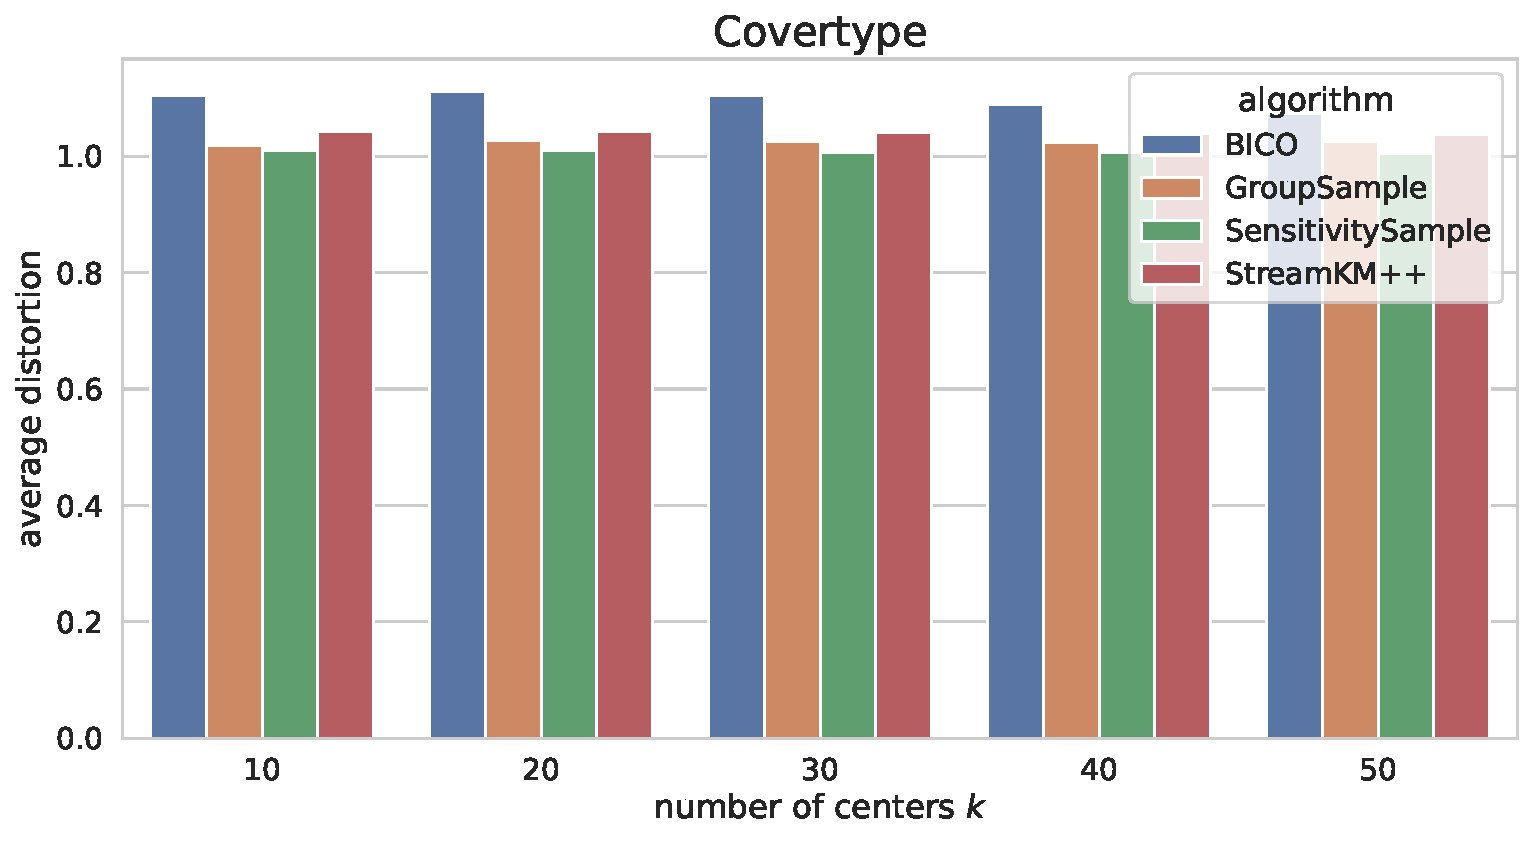
\includegraphics[width=0.5\textwidth]{figures/results-Covertype.pdf}
  }
  \subfloat{
    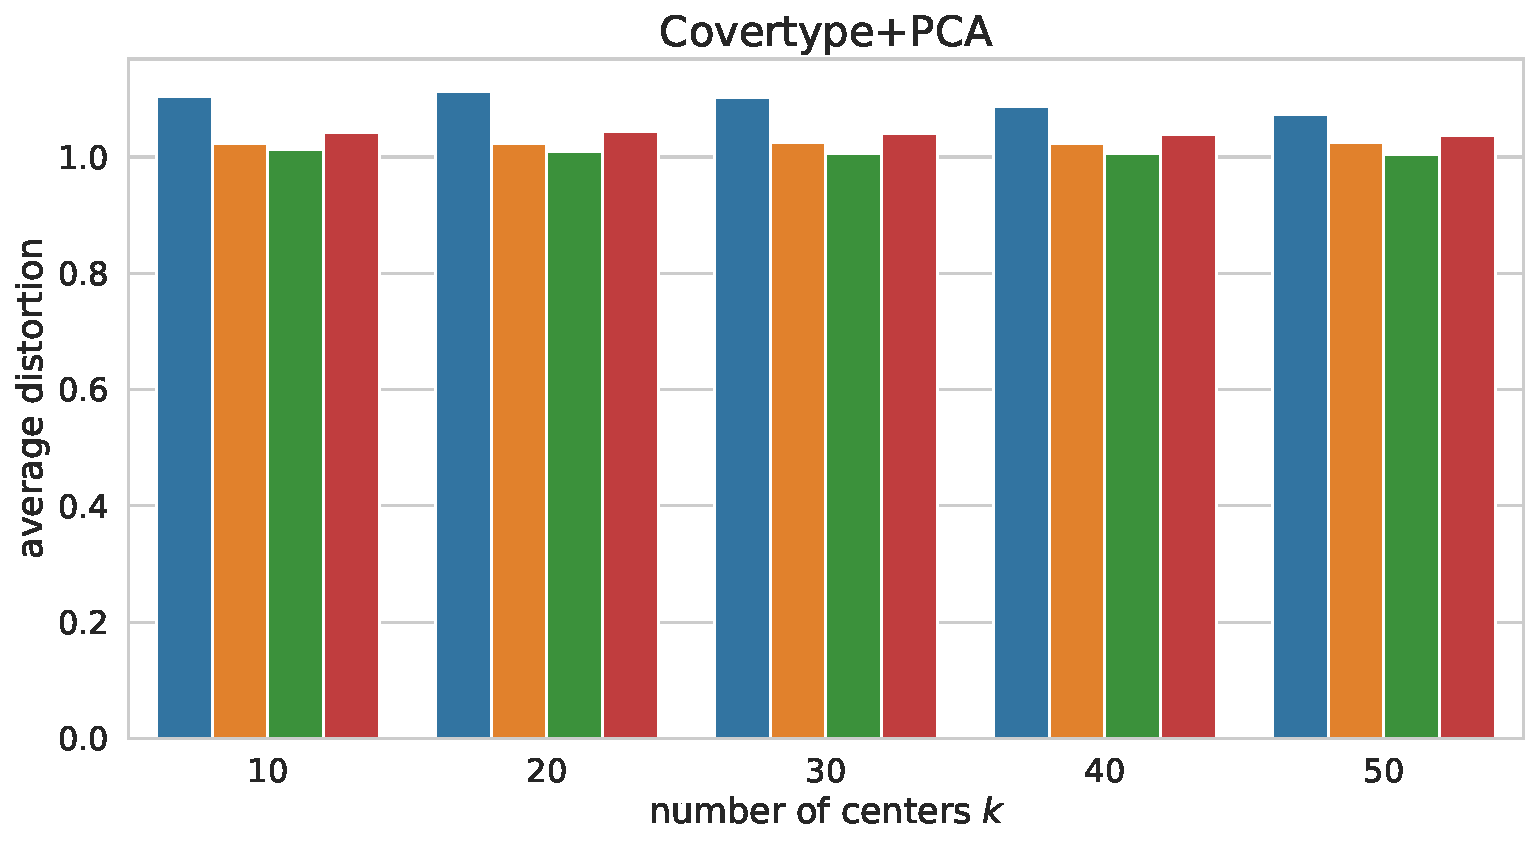
\includegraphics[width=.5\linewidth]{figures/results-Covertype+PCA.pdf}
  }
  \newline \newline
  \subfloat{
    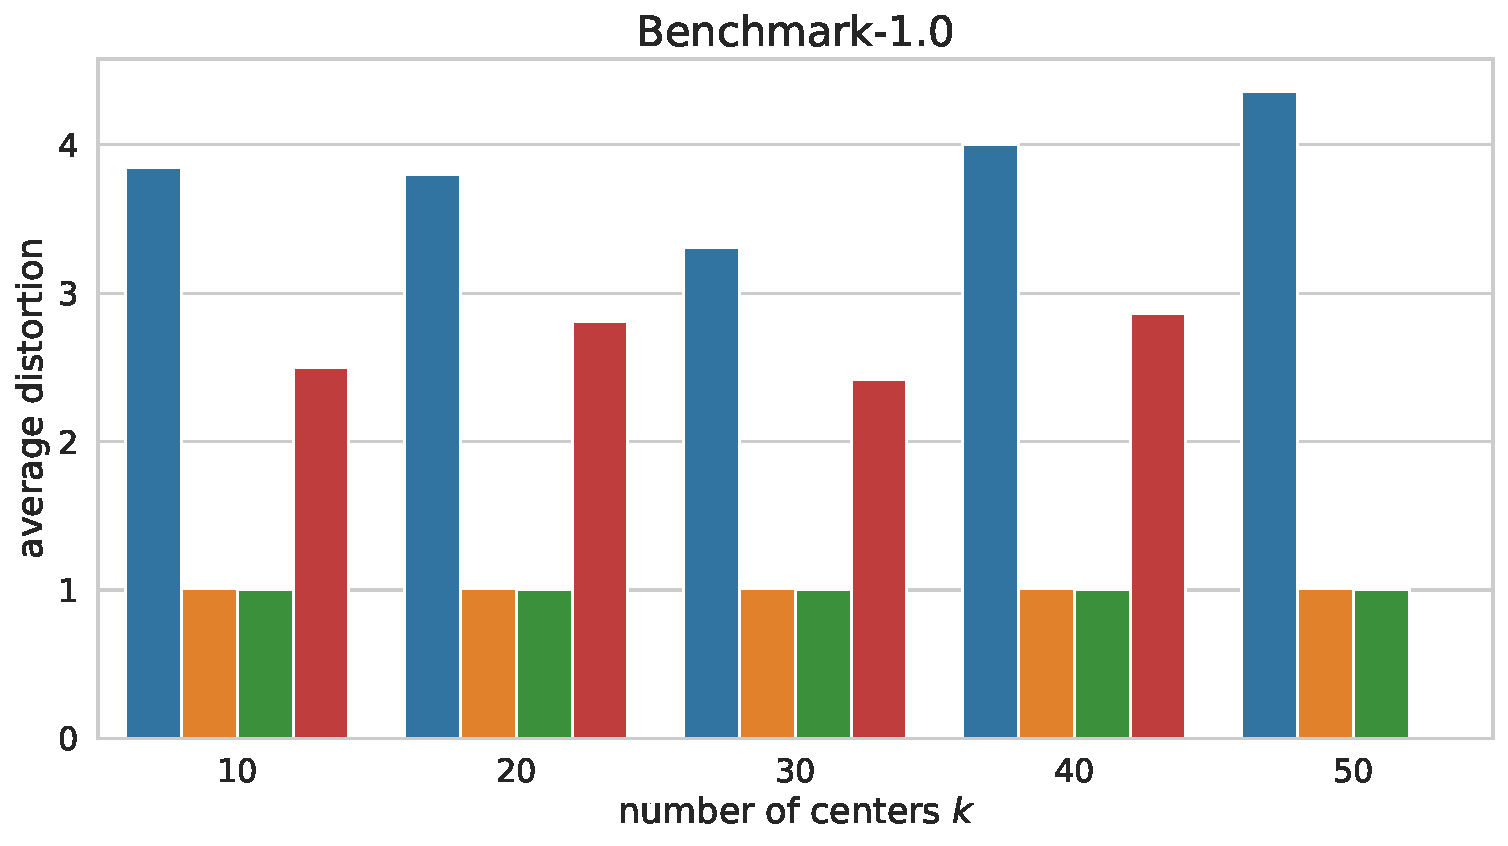
\includegraphics[width=0.5\textwidth]{figures/results-Benchmark-1.0.pdf}
  }
  \subfloat{
    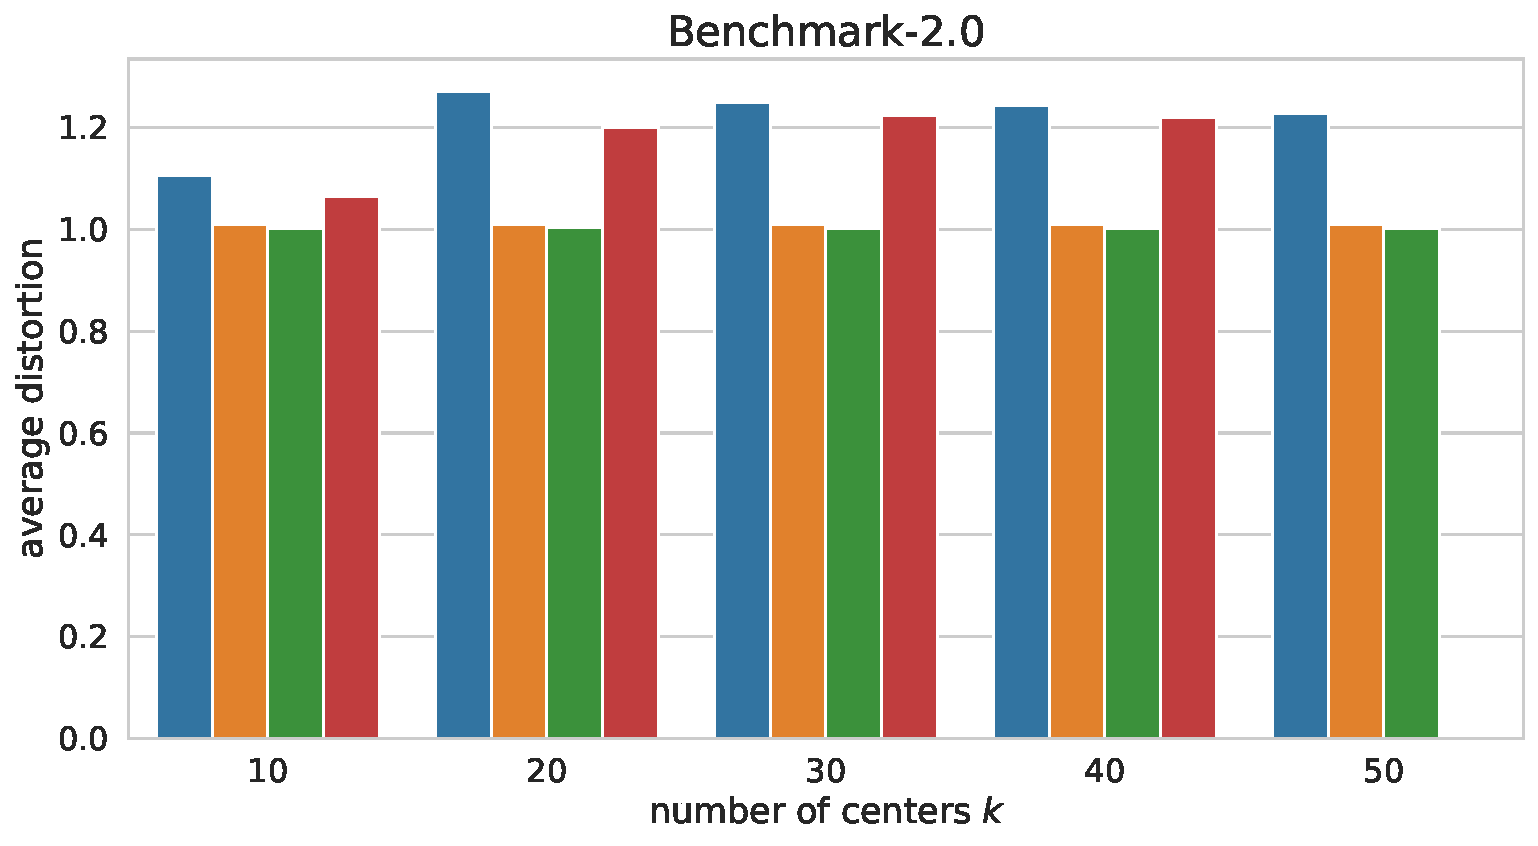
\includegraphics[width=.5\linewidth]{figures/results-Benchmark-2.0.pdf}
  }
  \label{fig:results}
  \caption{The results of the empirical evaluation of the four algorithms on different datasets.}
\end{figure*}
